%!TEX root = ../main.tex
\section{Networking}
The system deviced throughout this report seeks to ease the task of collecting data from the go-kart.
This is done by creating a network on the go-kart which allows the user to more easily add additional sensors.
In addition to providing a flexible platform for adding sensors, it will collect the data produced by the sensors on the network.
A goal with the project is to be able to monitor relevant data live through some interface.
To properly monitor data collected during driving it is necessary to maintain a live feed from the go-kart to the observer.
\\~\\
As mentioned above, there are two major functions to the system; recording of data and monitoring of data.
The recording is done on the go-kart using embedded hardware, specifically the Zybo platform is used to interface to the sensors.
The monitoring is done using a PC.
Monitoring is less time critical than the recording as it is simply meant for human readability.
For this reason, and to ease the workload, it has been decided to use a wifi connection between the go-kart and the PC.
Wifi, or even TCP/IP over ethernet is not viable on the go-kart between the Zybo boards due to the potentially long lag in that protocol.
A different network type will have to be devised for the embedded portion of the system.
This splits the network up into two parts, one that links the PC to the go-kart and one that links each component on the go-kart.
See figure \ref{fig:basic_network}.

\begin{figure}
	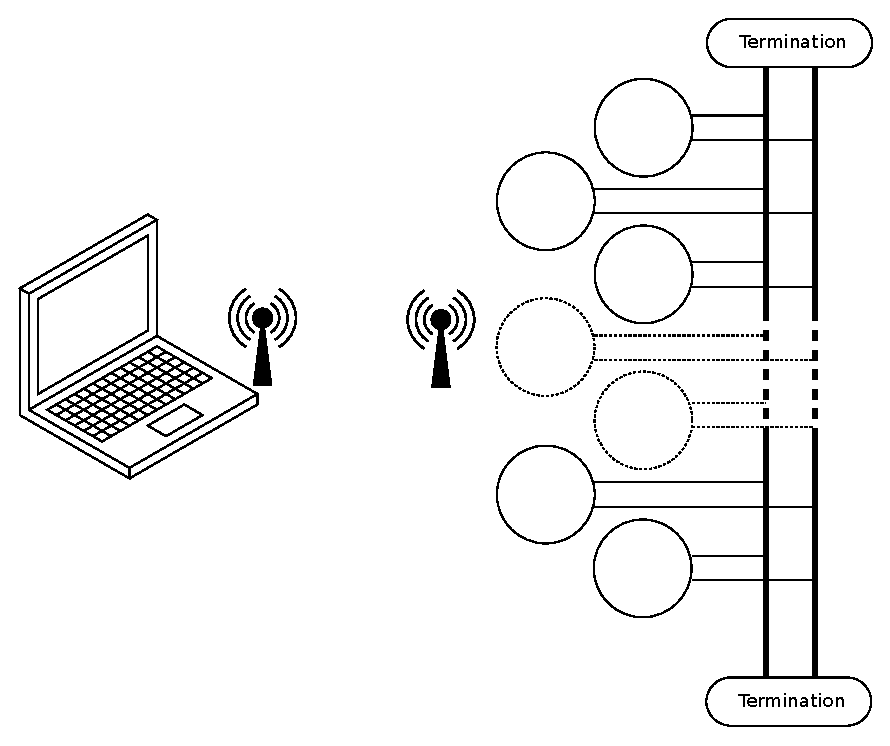
\includegraphics[width=.75\linewidth]{graphics/basic_network}
	\caption{A line of text}
	\label{fig:basic_network}
\end{figure}
\martin{I'm not sure this figure adds much understanding to the report}

These will be referred to as the off-kart network and the on-kart network, respectively, throughout the remainder of the report.
The following sections will explore the creation of both of these networks in turn.

\subsection{Off-Kart Network}
As mentioned above, the off-kart network is done using wifi.
It was chosen to use this method as all modern laptops are equipped with the capability of connecting to such a network.
Hereafter the challenge lies in establishing an ad-hoc network between a zybo board and a PC.
This network is created using the a USB-Wifi dongle on the Zybo board. 
The following script is run to bring down the device, change the network type to ad-hoc, bring up the device, create the ad-hoc network and, finally, assign an IP-address to the device.
\martin{bring down and bring up?}
Note: some commands require super user access.
For clarity, \texttt{sudo} is left out from all calls throughout this section.
\begin{lstlisting}
>>service network-manager stop
>>ip link set wlan0 down
>>iw wlan0 set type ibss
>>ip link set wlan0 up
>>iw wlan0 ibss join go-kart 2412
>>ip addr add wlan0 196.178.10.9
\end{lstlisting}
It is verified working using the ping command from both the Zybo board and to the PC and vice versa.
Below is a thorough description of the challenges encountered while setting up this device as well as a brief explanation of the choice of device.
\\~\\
Two methods were immediately available for use: A usb wifi dongle and a PMOD wifi interface.
As the name implies, the latter is designed to be compatible with the PMOD interfaces on the zybo board (and a range of similar boards offered by Digilent Inc.).
It converts TCP/IP to SPI and vice versa.
However, since the zybo boards are already running a linux distribution, it was decided to attempt connecting through the usb wifi dongle.
This decision marked the beginning of a long journey, the highlights of which are discussed below. 
\\~\\
The first step was to ensure that the correct drivers are present on the system.
The usb dongle is a TP-LINK TL-WN722N.
This device uses the Atheros AR9271 chipset and is on the list of supported devices for the ath9k\_htc driver on wireless.wiki.kernel.org.
Running \texttt{dmesg} prints the kernel log, revealing, amongst other things, what drivers are loaded.
\begin{lstlisting}
>>dmesg | grep ath
[10.329564] usb 1-1: ath9k_htc: Firmware htc_9271.fw requested
[10.332438] usbcore: registered new interface driver ath9k_htc
\end{lstlisting}
Additionally:
\begin{lstlisting}
>>lsusb | grep Ath
Bus 001 Device 002: ID 0cf3:9271 Atheros Communications, 
	Inc. AR9271 802.11n
\end{lstlisting}

\martin{is one ath supposed to be lower case and the other upper case in the listings above?}
As per these commands the operating system (OS) has correctly detected and loaded the driver.
The \texttt{iproute2} package contains the utilities used to manipulate TCP/IP connections.
\begin{lstlisting}
>>ip link show
1: lo: <LOOPBACK,UP,LOWER_UP> mtu 65536 qdisc noqueue 
	state UNKNOWN mode DEFAULT group default 
    link/loopback 00:00:00:00:00:00 brd 00:00:00:00:00:00
2: eth0: <BROADCAST,MULTICAST,UP,LOWER_UP> mtu 1500 qdisc pfifo_fast 
	state UP mode DEFAULT group default qlen 1000
    link/ether 00:0a:35:00:01:22 brd ff:ff:ff:ff:ff:ff
3: wlan0: <BROADCAST,MULTICAST> mtu 1500 qdisc mq 
	state DOWN mode DEFAULT group default qlen 1000
    link/ether ec:08:6b:1b:41:b3 brd ff:ff:ff:ff:ff:ff
\end{lstlisting}
\martin{We need to ensure, that the lines do not become wider than the textwidth}

The device has been given the identifier \texttt{wlan0}.
It can be brought up by:
\begin{lstlisting}
ip link set wlan0 up
>>ip link show wlan0
3: wlan0: <NO-CARRIER,BROADCAST,MULTICAST,UP> mtu 1500 qdisc mq 
	state DOWN mode DEFAULT group default qlen 1000
    link/ether ec:08:6b:1b:41:b3 brd ff:ff:ff:ff:ff:ff
\end{lstlisting}
At this point the device is up, as can be seen on the list of flags:
\begin{lstlisting}
<NO-CARRIER,BROADCAST,MULTICAST,UP>
\end{lstlisting}
However, the \texttt{NO-CARRIER} flag is also set.
This flag indicates a fault on the physical layer, i.e. a disconnected network cable or similar.
Running a scan on the device shows that it is able to correctly detect nearby networks:
\begin{lstlisting}
>>iw dev wlp2s0b1 scan | grep SSID
SSID: SDU-WEBLOGIN
SSID: eduroam
SSID: SDU-GUEST
\end{lstlisting}
This was believed to be a software related issue, as it could detect networks, but not correctly connect to them.
In an attempt to isolate the error the dongle was connected to a PC.
The dongle worked flawlessly on the PC and connected to the internet after bringing down the standard interface.
Clearly, there are differences between the two systems, one or more of which were causing one to work while the other did not.
In order to eliminate these differences the versions of the involved software was brought up to date.
The PC is running Arch Linux, a distribution using rolling release.
This means that, generally, the software will always be at the latest stable release.
The Xillinux distribution running on the Zybo board is based on the Ubuntu 12.04 release, the long term support version from 201, see \cite{xillinux}. \martin{which year?}
As such, much of the software is outdated.
The \texttt{iproute2} package as well as \texttt{network-manager} was updated to the latest version.
Other than provide some experience with building and searching for dependencies, it did little to alleviate the issues.
\\~\\
It was decided to continue attempting to set up the ad-hoc network on the PC, expecting that this process may provide some insight into the issues on the Zybo board, and how to fix them.
Initially the drivers were verified using the same procedure as mentioned previously, for brevity, this is left out.
From experience, the first step was to disable the network manager.
A network manager is particularly useful when a user wants to connect to the internet or similar, basic operations.
It automatically detects hardware and manages connections in the area.
The automatic setup means that it will often overwrite any changes made by the user.
For this reason the network manager is disabled:
\begin{lstlisting}
>>systemctl connman.service stop
\end{lstlisting}
\texttt{connman} is the network manager used on the system.
In order to create an ad-hoc network it is necessary to change the mode of the interface to IBSS (Independent Basic Service Set):
\begin{lstlisting}
>>ip link set wlp2s0b1 down
>>iw wlp2s0b1 set type ibss
\end{lstlisting}
Notice that the interface naming on this system is following the new "predictable network interface names"-scheme.
This scheme names the interfaces based on various factors such as MAC-address of the hardware, for more details see \cite{interfacenaming}.
The interface needs an address assigned to it in order to communicate on the network.
\begin{lstlisting}
>>ip addr add 192.168.10.9 dev wlp2s0b1
>>ip link set wlp2s0b1 up
\end{lstlisting}
Finally, after having brought up the device, the ad-hoc network can be created:
\begin{lstlisting}
>>iw wlp2s0b1 ibss join go-kart 2412
\end{lstlisting}
This commands creates an ibss (ad-hoc) network called go-kart on frequency 2.412 \si{\giga\hertz}.
Repeating these steps on a different system, assigning a different address to it, makes it possible to ping between the systems: 
\begin{lstlisting}
>>ping 192.168.10.11
PING 192.168.10.11 (192.168.10.11) 56(84) bytes of data.
64 bytes from 192.168.10.11: icmp_seq=1 ttl=64 time=0.592 ms
64 bytes from 192.168.10.11: icmp_seq=2 ttl=64 time=0.638 ms
\end{lstlisting}
Having this up and running, it was attempted to run the above sequence of commands on the Zybo board.
This allowed the Zybo board to correctly create the network.
Trying to ping the board on its assigned IP-adress, however, yielded a \texttt{no route to host} message.
Looking into the routing tables reveals a discrepancy:
\begin{lstlisting}
>>ip route show
default via 192.168.10.1 dev eth0 metric 100 
169.254.0.0/16 dev eth0 scope link metric 1000 
192.168.10.0/24 dev eth0 proto 
	kernel scope link src 192.168.10.10 
\end{lstlisting}
\thomas{Get the correct table, wifi is missing}
As can be seen, messages on eth0 and wlan0 are both routed to the same address space, 192.168.10.0/24.
Curiously, this did not pose an issue on the PC's.
Changing the address space to something different corrected the problem.
In this case 196.178.10.0/24 was chosen.
Finally, a short bash script is written to quickly set up the network:
\begin{lstlisting}
>>service network-manager stop
>>ip link set wlan0 down
>>iw wlan0 set type ibss
>>ip link set wlan0 up
>>iw wlan0 ibss join go-kart 2412
>>ip addr add wlan0 196.178.10.9
\end{lstlisting}
